\documentclass[LPM,lsstdraft]{lsstdoc}
\usepackage{enumitem}

\setDocChangeRecord{%
\addtohist{}{2018-03-24}{Initial version.} {WOM}
\addtohist{}{2019-02-25}{Added site topology schematic} {LPG}
%\addtohist{1.0}{2017-12-12}{Approved in \jira{RFC-xxx}.}{W.~O'Mullane, T.~Jenness}
}

\title[Independent DACs]{Proposed Policy for Independent Data Access Centers}

\author   {William O'Mullane, Beth Willman, Melissa Graham, Leanne Guy, Robert Blum }
\setDocRef      {LPM-251} % the reference code
\setDocDate     {\today}              % the date of the issue
\setDocUpstreamLocation{\url{https://github.com/lsst/LPM-251}}
%
% a short abstract
%
\setDocAbstract {
This document describes the proposed policies for groups that are independent from the LSST Project and Operations (i.e. LSST Data Facility) and would like to stand up an independent Data Access Center (iDAC; existing data centers that could serve LSST data products are considered iDACs for purposes of this document). Some iDACs may want to serve only a subset of the LSST data products: this document proposes three portion sizes, from full releases to a "light" catalog without posteriors. Guidelines and requirements for iDACs in terms of data storage, computational resources, dedicated personnel, and user authentication are described, as well as a preliminary assessment of the cost impacts. Some institutions, even those inside the US and Chile, may serve LSST data products locally to their research community. Requirements and responsibilities for such institutional bulk data transfers are also described here. {\bf The purpose of this draft document is to serve as a {\it preliminary} resource for partner institutions wishing to assess the feasibility of hosting an iDAC in the era of the Open Data Framework, and is subject to change.}
}
\graphicspath{ {./figs} {./images} }

\begin{document}
%
% the title page
%
\maketitle

\renewcommand{\thepage}{\arabic{page}}% Arabic numerals for page counter

\setcounter{page}{1}% Start page number
%\printnoidxglossaries
%
% It's all yours from here on
%
\section{Introduction}\label{sec:intro}


In 2019 LSST with NSF and DOE has considered that maximizing science is best achieved through an Open Data Framework (ODF).
Getting data to as many scientist as possible without restrictions will foster more collaborations and should give maximum science return. Gaia's \citep{2016A&A...595A...1G} open data policy has certainly shown this to be the case with around one thousand publications since the first data release. SDSS also had a open data policy and has over eight thousand publications since 2003 (DR1).
% not very well done ADS search restricted to staert from year 2015 for Gaia and 2003 for SDSS - number of refereed papers.
This is a departure from the previous LSST notion of proprietary data products.


 Access to LSST data products for any users will be possible through a Data Access Center (DAC). The United States's DAC will be hosted at the National Center for Supercomputing Applications (NCSA),
where authorized LSST users will perform scientific queries and those with sufficient privileges will be allowed to perform analysis on the full data releases using the LSST Science Platform (LSP). The LSP is now well documented with the vision given in \citeds{LSE-319}, with more formal requirements in \citeds{LDM-554} and the design in \citeds{LDM-542}. The Chilean DAC will be equivalent in functionality to the US DAC, but scaled-down in terms of the computational resources available for query and analysis given the smaller Chilean community \citedsp{LDM-572}\footnote{Most recently the Chilean Government has started the data observatory initiative \url{https://www.economia.gob.cl/data-observatory} which may see this DAC moved to the cloud}.

Within the ODF data products may be accessed from a host of other potential locations where one would normally expect to find astronomical data. This is discussed further in \secref{sec:public}


%This document proposes a set of guidelines and policies for partner institutions -- in the US, Chile, or one of the International Contributors with signed Memoranda of Agreement -- that are interested in hosting the LSST data, in whole or in part, for their affiliated members as an independent Data Access Center (iDAC).
The following sections include the types of data products that could be hosted (Section \ref{sec:data}), the requirements and responsibilities that would be expected of an iDAC hosting LSST proprietary data products (Section \ref{sec:reqs}), and a description of the main costs {\it vs.} their science impacts (Section \ref{sec:costs}).

The contents of this draft are meant to provide a preliminary resource for partner institutions who may be assessing the feasibility of hosting an iDAC. The specific mechanisms and processes by which future iDACs will negotiate the bulk transfer of data, the installation of software, etc. is considered beyond the scope of this document.

To help get an idea of sizes \tabref{tab:sizes} gives an overview.


\begin{table}
\caption{Size summary based on \citeds{LDM-141} \label{tab:sizes}}

\begin{tabular}{l r l r r r }
\hline
 \bf{Table}  &    \bf{Bytes/row} &\bf{Rows (DR1 -> DR11)} &\bf{DR1 (TB)} &\bf{ $\times$ Growth } &\bf{DR10 (PB)}\\
\hline
 Object\_Lite    &1840   &$2.26^{10} -> 4.74^{10}$ &42  &2.1  &0.08 \\
 Object\_Extra   &20393  &$2.26^{10} -> 4.74^{10}$ &461 &2.1  &0.9  \\
 Source          &453    &$4.51^{11} -> 9.01^{12}$ &204  &20.0 &4.0  \\
 ForcedSrc       &41     &$1.20^{12} -> 5.01^{13}$ &49  &42  &2.0  \\
 DiaObject       &1405   &$7.94^{08} -> 1.54^{10}$  &1.1  &19.4 &0.002  \\
 DiaSource       &417    &$2.26^{09} -> 4.52^{10}$  &0.9&20 &0.002 \\
 DiaForcedSource &49     &$1.50^{10} -> 3.01^{11}$  &0.7 &20  &0.001 \\
\hline
 \multicolumn{6}{l}{Year ~1   raw images:$ 3 PB$, tables:$\sim 1 PB$, half for Object\_Extra,$ 0.2 PB$  Sources}\\
 \multicolumn{6}{l}{Year 10   raw images:$ 30 PB$, tables:$\sim 7 PB$,$ 4 PB$  Sources,$ 2.0 PB$  Forced ,$ 1 PB$  Object\_Extra}\\
\hline
\end{tabular}
\end{table}


All access to, and use of, the LSST data and data products is subject to the policies described in \citeds{LPM-261}.



\section{Public Data - the Open Data Framework (ODF)}\label{sec:public}

The ODF simplifies the issue of data rights by effectively removing the proprietary period, as was done on Gaia,
\footnote{One should note from Gaia a small tone of discontent summed up in \url{https://blogs.scientificamerican.com/observations/the-price-of-open-science/}},
and making the data public.

With public data be we face a potential huge number of users.
Alex Szalay at AAS noted there were over a million unique IP addresses which hit the SDSS archive over a one year period.  Gaia saw 2K users accounts per hour on the catalogue release - we are clearly not only serving the 10K professional astronomers in the world anymore.
This could be mitigated in two ways.


Nationally we could partner with Google or Amazon who will notionally host public data sets for free - so we could more selectively add users to the DACs and try to put most casual users to the public interface. It is not clear if this would then be the EPO interface but that is worth considering i.e. EPO would no longer have to select 10\% of data but it would have a much bigger job to deal with all of it perhaps.
The public data set would be some lite version for the catalog \secref{sec:lite}  and the HiPS type color images. No raw data files and potentially no advanced notebook type access. This may not even need a logon for the fast queries like show me M31 with LSST sources plotted. This would not include the source catalogue which is the big one ($10^{13}$ rows).
Potential national partners  could also host the object catalog e.g.

\begin{itemize}
 \item MAST at STScI
 \item DataLab at NOAO
 \item SAO
 \item US Naval Observatory
 \item NED at IPAC
 \item HEASARC
 \item CADC - Canadian Astronomical Data Centre - we work with them already in Data Management.
\end{itemize}

\subsection {International}
Internationally we could partner with s network of sites - it should be a network to allow peer to peer sharing of catalogs. Here we could provide the HIPS color images and again some version of the OBJECT catalogue. We would have to consider if the source catalogue should also be distributed to a smaller subset of centres who could cope with it.
Potential International Partners might be:

\begin{itemize}
\item In Europe we have a few centres that Astronomers expect to find sources at:
\begin{itemize}
    \item CDS  - Aladin and Vizier - this is a minimum for Europe
    \item ESAC - ESASky - European Space Agency
    \item  ASDC - Italian Data Center
    \item  GAVO MPA - German Astronomical Virtual Observatory - Max Plank Astrophysics
    \item  IoA - Cambridge
    \item  Edinburgh
\end{itemize}
\item In Asia
\begin{itemize}
    \item  NAOJ Astronomical Data Center, Tokyo
    \item  Chinese Academy of Sciences - perhaps National Space Science Center
\end{itemize}
\end{itemize}


Having the lite catalog hosted at multiple locations where, and in formats which, astronomers would expect to find catalog information would reduce load on the US and Chilean DAC.
 It will also put the LSST data more readily in the hands of the astronomers and should accelerate science at least in the cases where the catalog is the prime source of information e.g. galactic dynamics and other large statistical studies.


\section{Types of Data Products for IDACs}\label{sec:data}
% Operations-era language for data products, as defined in  LSE-231, should be used

The three categories of LSST data products, {\it Prompt}, {\it Data Release}, and {\it User Generated} are defined in the LSST Data Product Categories document  \citeds{LPM-231}.
Both the {\it Prompt}, {\it Data Release} data products are produced by LSST and include images, both raw and processed, and catalogs of both {\tt Object}s and {\tt Source}s.
The  {\it User Generated} data products are produced the community using the resources of the LSST Science Platform \citeds{LSE-319}.
These data products are described in detail in the Data Products Definitions Document \citeds{LSE-163}.

Below, three potential realizations of the the LSST {\it Data Release} data products that IDACs might consider hosting are described: the full {\it Data Release} including images, the {\it Data Release} catalogs only, and a low-volume (``{\tt lite}'') subset of the {\it Data Release} catalogs.

\subsection{Full Data Release(s)}

In this case the IDAC would be hosting all of the raw and processed images, and catalogs, as described in \citedsp{LSE-163}. Hosting the raw image data at an IDAC requires roughly $6$ petabytes per year of storage, so this represents a significant augmentation of resources in terms of both hardware and personnel. The processed data and associated calibrations bring the total data volume to $0.5$ exabytes for a single data release. Some data volume could be saved by taking only a single calibrated image per band, but the total would still be $60$ petabytes (with compression it may be possible to reduce this even further). Any IDAC considering hosting the full {\it Data Release} should also deploy the full LSST Science Platform \citeds{LSE-319} in order to maximize science productivity and their return on investment in hosting an IDAC.

\subsection{Catalog Server}

Alternatively, an IDAC may find that hosting only the {\it Data Release} catalogs, and not the images, is sufficient for the scientific needs of its community. This will probably require the specific LSST database server \citedsp{LDM-135} and specific machines, and the deployment of the database system and the associated subset of data access services (DAX; e.g., web APIs, Qserv, \citeds{LDM-152}). The full {\tt Object} catalog, which contains one row per object with a volume of $\approx 20$ kilobytes per row, is estimated to contain about $40 \times 10^9$ objects (even in the first full-sky data release). Adding to this the full {\tt Source} and {\tt Forced Source} catalogs, which contain one row per measurement in each of the $\sim80$ visit images obtained per year, brings the total storage volume required up into the petabytes range, and will require a serious commitment of resources at the proposed IDAC. The evolution of catalog sizes over the 10-year LSST survey is depicted in \figref{fig:catvol}, from which it is evident that the catalog size for the final release is order $15$ petabytes. For more details on the row counts see the Key Numbers Page\footnote{\url{https://confluence.lsstcorp.org/display/LKB/LSST+Key+Numbers}}.

\begin{figure}
\begin{center}
\includegraphics[width=0.8\textwidth]{images/CatVolTime.png}
\caption{Catalog volume over time from \citeds{LDM-144}. \label{fig:catvol}}
\end{center}
\end{figure}

\subsection{An ``{\tt Object Lite}" Catalog}\label{sec:lite}

Many -- perhaps most -- astronomers' science goals will be adequately served by a low-volume subset of the {\tt Object} catalog's columns that do not include, for example, the full posteriors for the bulge+disk likelihood parameters.
This {\tt Object Lite} catalog would nominally contain $1840$ bytes per row for the $40 \times 10^{9}$ objects, giving a size of $\approx 7.4 \times 10^{13}$ bytes ($\sim74$ terabytes).
Even smaller, science-specific versions of {\tt Object Lite} could be envisioned with even less columns and/or separate star and galaxy catalogs.
The Solar System community for example will be primarily be interested in the contents of  just the  {\tt SSObjects} table.

These would not be small enough to handle on a laptop, but might be served by a small departmental cluster.
Searching even a small {\tt Object Lite} catalog would require some form of database, but many institutes would already have a system which may be capable of loading this data.
In this case, LSST might only ship files with documentation and not provide administrative support for the system, but this would allow the {\tt Object Lite} catalog to be widely available to all partner institution IDACs. Distribution options such as peer-to-peer networking to avoid download bandwidth limitations might be possible to implement in this case.
%See also \secref{sec:public}.


% LPG Detail here the minimum resources and levels of service that a iDAC must commit to to be qualify for consideration as an LSST iDAC
% I wouldn't call this guidelines - there are concrete requirements that must be met

\section{Requirements and Guidelines for iDACs}\label{sec:reqs}
Since creating, delivering, and supporting the implementation of LSST data products in iDACs creates some cost to the LSST Project, iDACs will be expected to follow some basic requirements and guidelines that are described below.
The actual costs of iDAC support and infrastructure development are considered separately in Section \ref{sec:costs}.



\subsection{LSST site topology} \label{sec:topology}

{\color{red}Leanne to describe the flow in the topology diagram.} \newline

\begin{figure}
\begin{center}
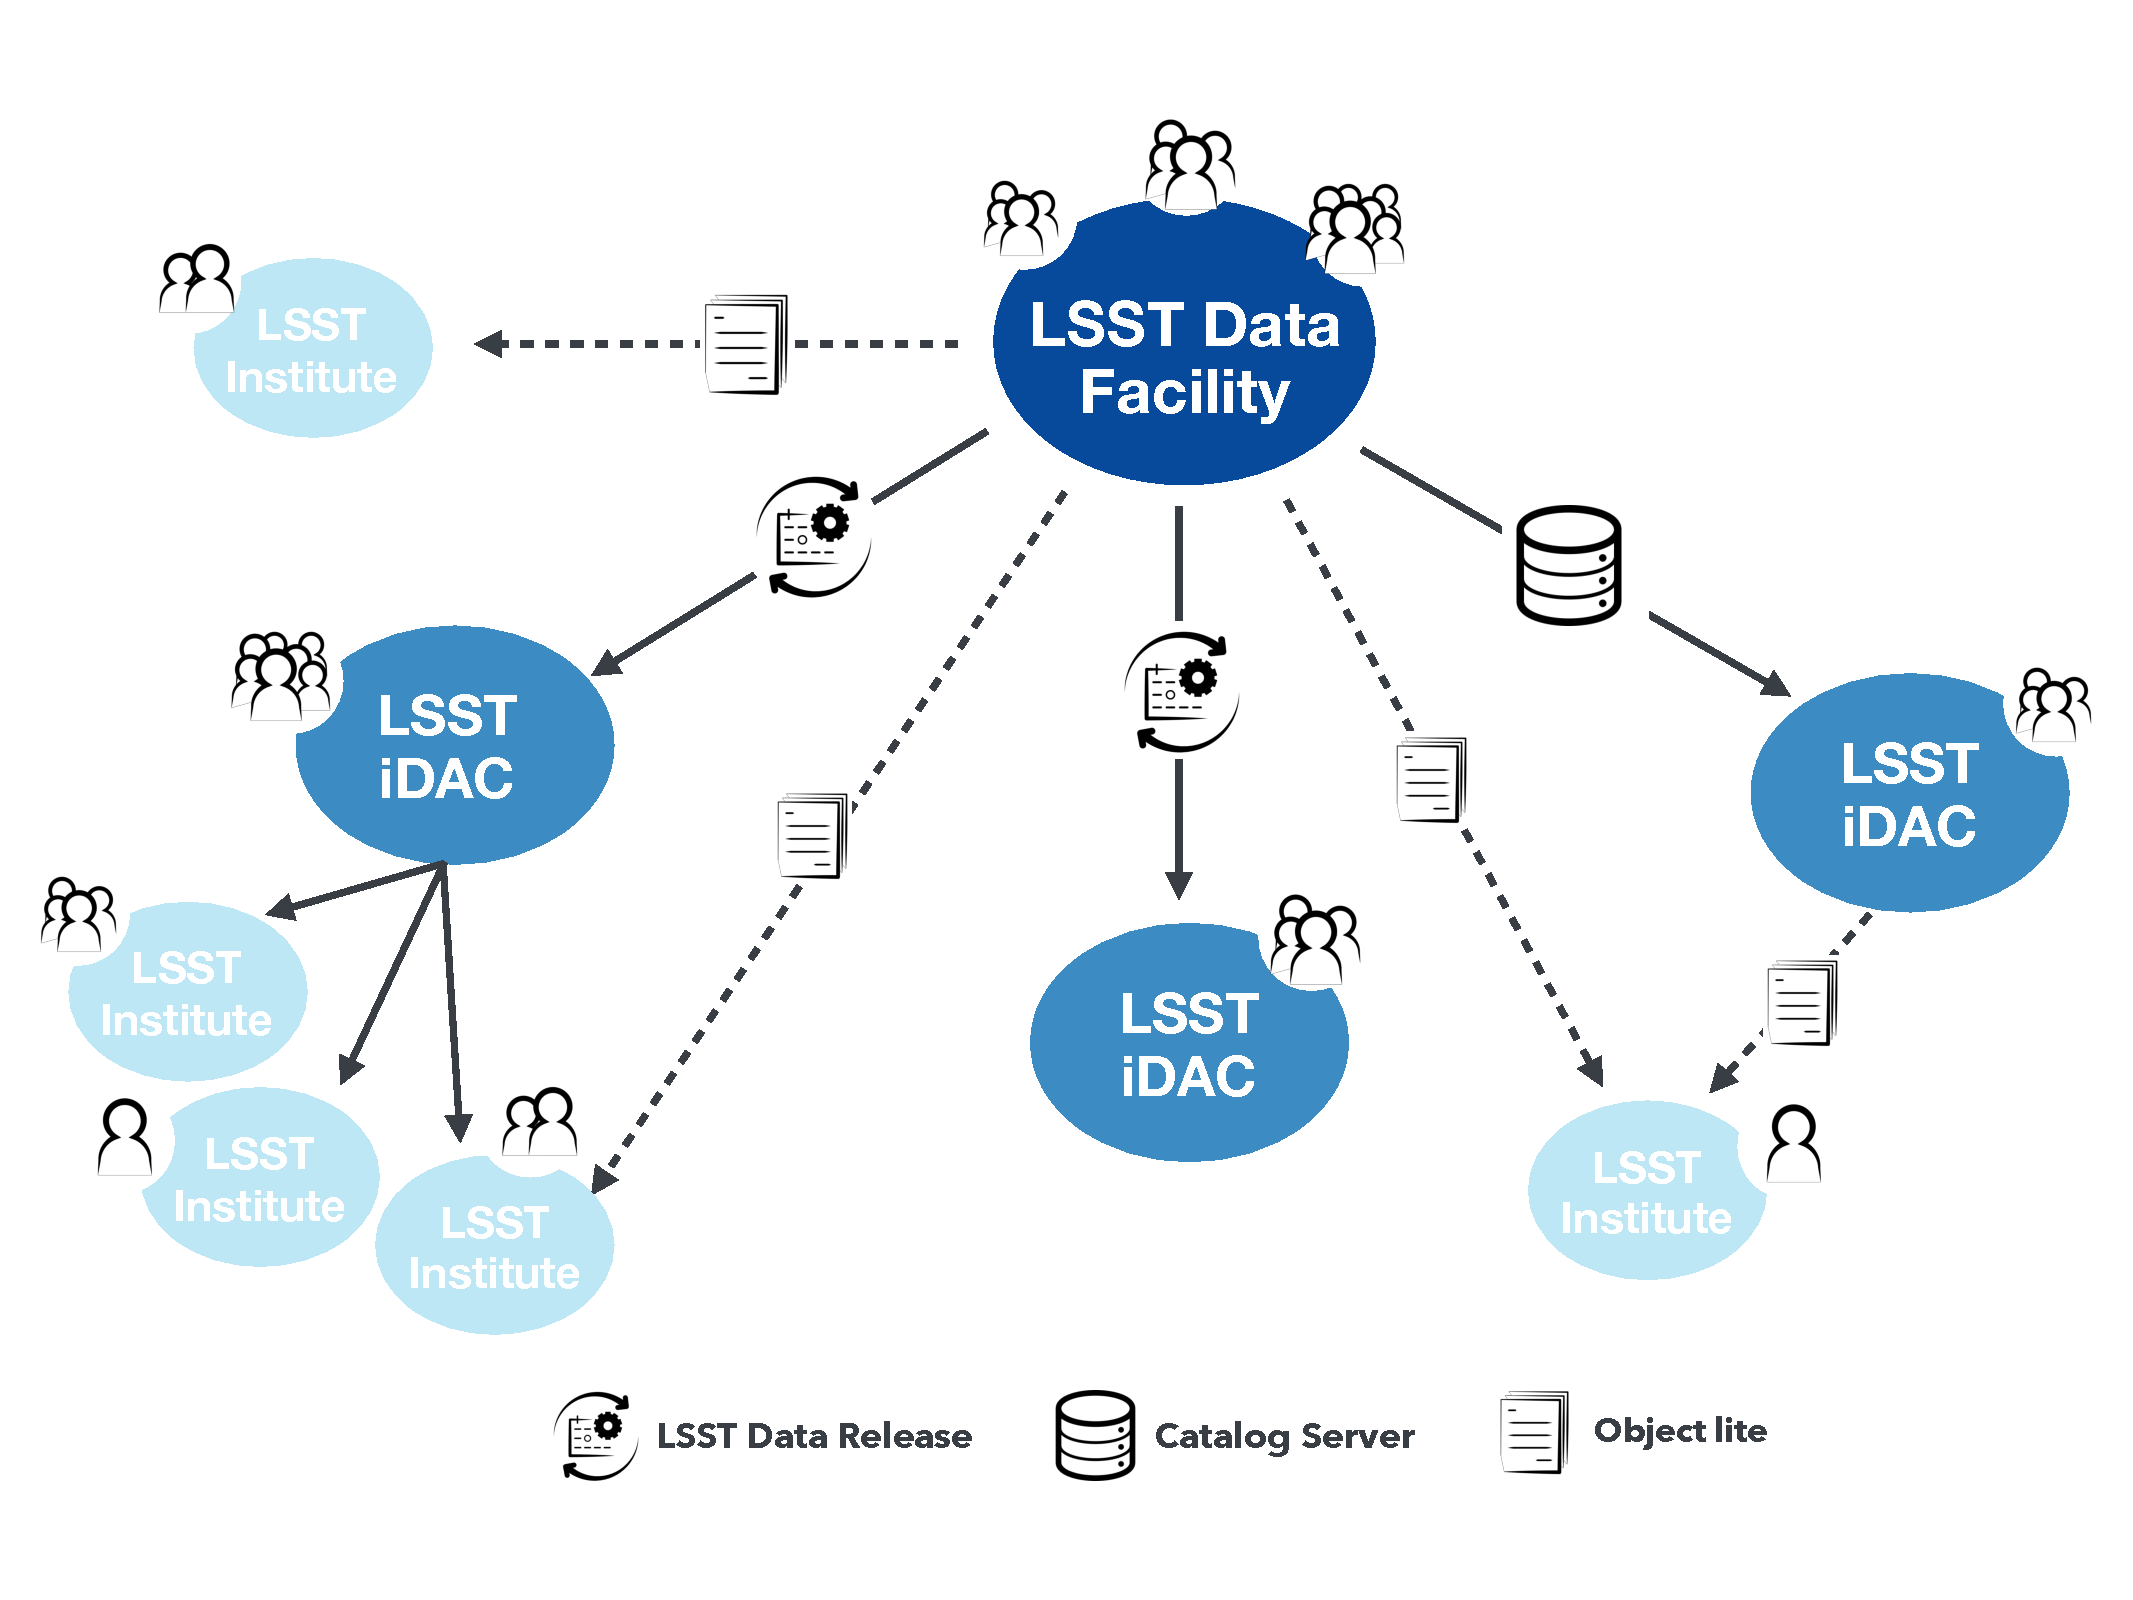
\includegraphics[width=0.8\textwidth]{images_local/LSST-site-topology}
\caption{LSST Data Facility and Independent DAC network topology.  \label{fig:lsst-site-topology}}
\end{center}
\end{figure}



\subsection{Required Resources} \label{sec:resources}
Institutions or organizations wishing to set up independent data access centres will be expected to have
sufficient resources and commitments before we discuss data transfers and support.
See also \secref{sec:cvs} for a discussion on compute vs storage.
%Perhpas that should move here

\subsubsection{Data Storage}
Any institution considering setting up an iDAC will need to show commitment on purchasing sufficient storage and CPU power to hold and serve the data. Sufficient storage ranges from $0.5$ exabytes for the full data release(s) down to $100$ terabytes for a catalog server, and potentially further down to $70$ terabytes if the {\tt Object Lite} option is offered. For the full catalog it is order 100 nodes to serve it up, and to serve images a DAC would need some additional servers; depending on load this may be order 10 additional nodes.

\subsubsection{User Computational}
If the full set of data release products including images and catalogs are desired, it is highly recommended that the iDAC deploy the LSST Science Platform (LSP). The LSP serves as a portal to the data, and provides a user interface of web services and Jupyter notebooks for scientific queries and analysis, an open software framework for astronomy and parallel processing, and the associated computational, storage, and communications infrastructure needed to enable science. The LSP is described in full in \citeds{LSE-319} and \citeds{LDM-554}. Depending on the assumed load, the LSP is relatively modest as it requires only $\sim2$ servers to set up, and it is recommended to have 2 CPUs per simultaneous user (e.g., if the iDAC's desired capability is to serve 200 users, but only expect 50 to be active at a time, then 100 CPUs would be sufficient). From that starting point, the amount of next-to-the-data computational resources can be as large as the data center wishes to provide, and may make use of connecting to e.g., local super computer resources.

\subsubsection{Dedicated Personnel}
The significant hardware required by an iDAC is above the normal level for most astronomy departments, and would require dedicated technical personnel to set it up and keep it running. For an {\tt Object Lite} catalog running on existing hardware, this might not be a significant increase in person power if the hardware is already serving on order $50$--$100$ terabytes. Still, it is recommended to assume $\gtrsim0.25$ full-time equivalent (FTE) personnel hours for {\tt Object Lite}, and perhaps closer to $\sim2$ FTE for the full catalogs, which includes setting up and maintaining the service, and installing new data releases and software updates every year. For iDACs wishing to host the full data releases' images and catalogs and deploy the LSST Science Platform, it becomes necessary to employ $1$--$2$ storage engineers to mange the large amount of data, and possibly one more FTE to keep the Kubernetes (or equivalent) system updated with the latest software deploys. If the iDAC intends to support the science of many local users, support will become a specific issue which may not be covered by the usual institutional funding, and will require further effort. It is therefore recommended that any partner institution wishing to host a full-release iDAC provide a minimum personnel of 5 FTE to be considered viable.

\subsection{Networking and distribution}
There is an assumption than any prospective iDAC will have a high bandwidth connection with demonstrated sustained $40 Gb/s$ to enable data transfer ans sufficient bandwidth for access by users.
In addition all iDACs should be ready  to serve the 'object-lite' catalog to any institution worldwide but especially any {\em local} institutions.

\subsection{Services}
{\color{red} Leanne } \newline

Services provided by LSST partner iDACs

\subsubsection{The LSST Science Platform}
All LSST independent data access centres must run an instance of the LSST Science Platform

\subsubsection{User Generated data products }
% Detail here the responsibilities and commitments of the LDF to LSST iDACs. See annex 3.1

% LPG Outline the responsibilities of the LDF towards recognized iDACs
\section{Responsibilities of the LSST Data Facility}

<<<<<<< HEAD
This section describes the services that the LSST Data Facility (LDF) will provide in support of all LSST iDACs.

The LDF will prepare data products for distribution to iLSST DACs along with documentation of hardware and software that will make serving these data consistent with the serving of data from the LSST DACs. LSST will provide (modest) technical support consistent with available resources to assist groups setting up iLSST DACs. 
=======
% redundant with title.. This section describes the services that the LSST Data Facility (LDF) will provide in support of all LSST iDACs.
>>>>>>> f24d03a705acc3cd3087a938815e2badc9fe6eb4

The LDF will prepare data products for distribution to along with documentation  including documentation of  software  and indicative hardware that will make serving these data consistent with the serving of data from the LSST DACs.

<<<<<<< HEAD
All LSST  iDACs must be able to serve the 'object-lite' catalog to any institution worldwide.

\subsection{Proprietary Data Access Policies}
{\color{red}Defer for now until further guidance received.} \newline
=======
LSST will provide (modest) technical support consistent with available resources to assist groups setting up non-LSST DACs provided the comply with prerequisites discussed in this document and especially in \secref{sec:resources}

\subsection{Data Distribution} \label{sec:dist}

NCSA will have $100Gb/s$ connections  on ESNET which has interconnects with Internet2 - this should provide a distribution mechanism for getting data to iDACs, it will however be limited by the fact that much of our bandwidth is already allocated for data transmission to IN2P3 and alert distribution.

A tiered model as used by CERN for high energy physics would seem a desirable way to achieve big transfers. Hence we would have a small selection of tier 2 centres with all data products from which tier 3 centres could copy the subsets they wish to work with.  Other alternatives are discuss in \secref{sec:xfer}.
>>>>>>> f24d03a705acc3cd3087a938815e2badc9fe6eb4

In HEP experiments such as  BABAR various physics analysis groups (science collaborations in LSST ) were assigned to specific international centers as their primary computing and analysis facility, thereby distributing the computing load around the "network". People naturally tend to use the facility with available resources and cycles anyway of course.
National groups received credit against their normal "operating common fund" contributions (equivalent to part of the LSST operations cost) based on their local computing contribution, and service to the full collaboration (equivalent to the full LSST data rights community).
We have not discussed  such system in place for LSST yet though.
~
%WOM - I took a go at it ..
%Points to be addressed
%\begin{enumerate}
%\item High-bandwidth network out of the LDF to all iDACs
%\item Distribution of each of the data products types outlined in \ref{sec:data} to iDACs
%\item ......
%\end{enumerate}



%l
%%%MLG: commented this out (WOM, delete if we'll never need to say this).
% It remains an open question whether {\em any} qualified user from any LSST partner institution can log into any iDAC -- this would facilitate collaboration but would also require that iDACs participate in the single authentication system.

%%%MLG: commented this out (WOM, delete if we'll never need to say this).
\subsection{iDACs Serving Post-Proprietary Data}
% {\bf MLG: can we think of any requirements/guidelines for this scenario? Should this document even cover non-partner iDACs? Any non-partner iDAC wishing to serve the two-year-old post-proprietary full release to its users would not, for example, be able to get help installing the LSP. Perhaps we could use this paragraph to further encourage the benefits of partnership.}

\section{Cost Impacts}\label{sec:costs}

As previously mentioned, standing up and maintaining multiple IDACs comes at a significant cost impact to both the LSST Project and the partner institutions. Minimizing these costs -- or at least maximizing the amount of science they enable -- should be at the forefront of all considerations concerning partner IDACs, such as the following propositions.

\subsection{Maximizing Profits with Science-Driven IDACs}
There are two main cost impacts of IDACs being set up outside of the US and Chilean DACs: the positive impact is that some computational load may be taken off of these existing DACs, but the negative impact is the level of support required from the LSST Project in order to get them set up and running. This negative impact could be mitigated by ensuring that science productivity is maximized as a result of this extended effort. One way to do this might be to associate specific areas of science to a given IDAC, and encourage users working in that field to use that IDAC. This could create a customer base for the IDAC, bring together like-minded experts, and effectively distribute the computing load across a network of IDACs. This might also enhance internal funding arguments for investment resources by arguing for synergies with local science goals and attracting international users and official endorsement.

\subsection{Data Transfer}\label{sec:xfer}
Even with good networks the data transfer will not be trivial, and could be quite expensive. LSST is not currently set up to distribute data to multiple sites, i.e., there is no form of peer-to-peer sharing. The bandwidth at NCSA is adequate for receiving data and delivering {\tt Alerts} to brokers during the night; perhaps some day time bandwidth could be used to transfer data to IDACs. A full data release of images and catalogs does not have to transferred within a given day; if the correct agreements are in place with an IDAC, a full release could be transferred slowly as it is produced, and then made available to the IDACs users in whole on the official release day.
\subsubsection{Transfer cost use case \label{sec:xfercost}} 
If we take the final number from the key numbers page \footnote{\url{https://confluence.lsstcorp.org/display/LKB/LSST+Key+Numbers}} we could consider DR1 as about 6 PB (10\% of the final size).

We would have at least  two ways to transfer this : via the network, via physical devices.

A network transfer at 10Gbps of 6 PB would take $8 * 6 \times 10^{12} \ 10^7 = 4.8 \times 10^{6}~seconds $ or about 55 days\footnote{ day = 86400}.
Many institutes have 100 Gbps connections so this should be an upper limit and a transfer should be order one week. If we had a peer to peer network this may go down somewhat and we may be able to support it from NCSA.

Alternatively we could host the data on Amazon or Google and let people download it from there - they would have more capacity.
Storage on the cloud  for public data would be theoretically free - download (egress)  would  cost.
Transfer to another cloud \footnote{\url{https://cloud.google.com/storage/pricingi\#network-pricing}}  or
 a Content Delivery Network (CDN)\footnote{\url{https://cloud.google.com/cdn/pricing}}
 end up costing  about a cent a GB which for an open science project and at our volume  should  be negotiable.  At one cent a transfer would cost
  $\sim \$0.01 * 6 \times 10^{12} \ 10^6 = \$60K$.

For physical devices, today apparently we could get a device like Petarack \url{https://www.aberdeeninc.com/petarack/} for \$300K.
Theoretically we could get this cheaper though this is close to the drive price,
Tape may also be a possibility especially if Sony/IBM commercialize high density tape with >300TB per cartridge\footnote{\url{https://newatlas.com/sony-ibm-magnetic-tape-density-record/50743/}}. A current 6TB cartridge is about \$30, so enough tapes for 6PB would cost about  30K. If the density increased this could come down significantly.
This could be be a partner data center cost as well as shipping it. Transfer of data on to this would be about the same as the network rate above so 7 days. SneakerNet \cite{2002cs........8011G} may still be  cost effective in the LSST era, which is predicted in the a paper.




\subsection{Compute {\it vs.} Storage Resources} \label{sec:cvs}
Data storage is a large cost to IDACs, and could be considered as an overhead relative to the amount of computational resources an IDAC can offer. If an IDAC is set up without a large compute capacity, the facility might be less useful to the science community than e.g., augmenting an existing DAC or IDAC to have more computational resources. It is conceivable that a partner institution may prefer to spend their money increasing the computational quotas available for a given collaboration or set of PIs, and it would be scientifically beneficial if this was possible at all DAC and IDACs. The notion of standard compute quotas and resource allocation committees to adjudicate on large proposals for substantial increases to computational allocations are described in \citeds{LDO-13}. Another way to approach a solution to this issue might be to have a \emph{Cloud}-based IDAC where a user or PI could buy nodes on the provider cloud to access the holdings put there by LSST.  Such an option may be particularly useful to Science Collaborations with large compute needs.

The full sizing model is in \citeds{DMTN-135} - any IDAC should have a similar sizing model. They may not need as much compute or as many copies of data as we have but the raw information to make such calls are in the technote.  For ball park figures the construction
to first year of ops table is copied here as tabref{tab:Summary}\footnote{ There is no guarantee of being in sync with \citeds{DMTN-135} but as an order of magnitude it is good.}.

%copied from DMTN-135 and modified
\tiny \begin{longtable} { |p{0.22\textwidth}  |r  |r  |r  |r  |r |}
\caption{This table from \citeds{DMTN-135}pulls together a high level summary  of costs using conservative price factors.
 \label{tab:Summary}}\\
\hline
\textbf{Year}&\textbf{2020}&\textbf{2021}&\textbf{2022}&\textbf{2023} \\ \hline
{Compute (2019 pricing)}&{\$690,000}&{\$0}&{\$1,510,000}&{\$2,820,000} \\ \hline
{Storage (2019 pricing)}&{\$190,702}&{\$126,563}&{\$1,216,867}&{\$7,864,125} \\ \hline
{Qserv (2019 pricing)}&{}&{}&{\$560,000}&{\$3,240,000} \\ \hline
\textbf{Total (2019 pricing)}&\textbf{\$880,702}&\textbf{\$126,563}&\textbf{\$3,286,867}&\textbf{\$13,924,125} \\ \hline
{Compute (applying price factor)}&{\$621,000}&{\$0}&{\$1,057,000}&{\$1,692,000} \\ \hline
{IN2P3 (50\% of compute in ops)}&{}&{}&{}&{-\$846,000} \\ \hline
{Storage (applying price factor)}&{\$181,167}&{\$113,907}&{\$1,034,337}&{\$6,291,300} \\ \hline
{Qserv (applying price factor)}&{}&{}&{\$434,000}&{\$2,268,000} \\ \hline
{Hosting cost NCSA
}&{\$110,802}&{\$62,802}&{\$238,012}&{\$536,801} \\ \hline
\textbf{Total budget (using price factors)}&\textbf{\$912,969}&\textbf{\$176,709}&\textbf{\$2,763,350}&\textbf{\$9,942,100} \\ \hline
\end{longtable} \normalsize



\appendix
\section{References\label{sect:references}}
\renewcommand{\refname}{}
\bibliography{local,lsst,lsst-dm,refs,books,refs_ads}

\section{Acronyms}
\addtocounter{table}{-1}
\begin{longtable}{|l|p{0.8\textwidth}|}\hline
\textbf{Acronym} & \textbf{Description}  \\\hline

CDN & Content Delivery Network \\\hline
CPU & Central Processing Unit \\\hline
DAC & Data Access Center \\\hline
DAX & Data access services \\\hline
FTE & Full-Time Equivalent \\\hline
GB & GigaByte \\\hline
GB & Giant Branch (star) \\\hline
IT & Integration Test \\\hline
LDM & Light Data Management \\\hline
LPM & LSST Project Management (Document Handle) \\\hline
LSE & LSST Systems Engineering (Document Handle) \\\hline
LSP & Low System Priority \\\hline
LSST & Large Synoptic Survey Telescope \\\hline
NCSA & National Center for Supercomputing Applications \\\hline
PB & PetaByte \\\hline
PB & Play-Back \\\hline
PI & Principle Investigator \\\hline
US & United States \\\hline
s & second; SI unit of time \\\hline
\end{longtable}
 % generated by the acronyms.csh (GaiaTools)
\end{document}




